\section{System: From Research Pipeline to Production Audit Console}\label{sec:system}\label{sec:production}

The preceding sections establish a narrow, defensible research claim about topology's marginal value under leakage-free evaluation. That claim is deliberately silent on whether the resulting models can run anywhere near a real ledger. Continuous-auditing research has long argued that a control is only as useful as the workflow that consumes it~\cite{vasarhelyi2012acceptance}, and post-implementation audits of ERP deployments routinely find that analytically sound models never reach production because the serving path, the data-integrity guarantees, and the operational evidence were never engineered~\cite{mamakou2024postimplementation}. This section describes what was actually built to close that gap: a Procure-to-Pay ERP core with a forensic audit console in front of it, an online scoring service that reuses the research pipeline's own feature-computation classes rather than reimplementing them, database-enforced financial-integrity invariants that do not trust application code to behave, and a measured (not assumed) performance and reliability profile. Every number in this section is either read directly from a project artifact file or drawn from a documented, reproducible test run; none are projected.

\subsection{Architecture Overview}\label{sec:system-arch}

The application is a conventional three-tier system chosen for auditability over novelty, consistent with the broader finding that ERP-adjacent ML systems succeed or fail on integration discipline more than on model sophistication~\cite{jawad2024erp}. A FastAPI backend exposes the ledger's domain objects (vendors, AP invoices, payments, payment runs, GL accounts, journal entries, audit alerts) through versioned REST routes (\texttt{app/api/\{vendors,invoices,payments,gl,alerts,auth,system\}.py}), backed by a normalized PostgreSQL schema and a Redis layer used for both response caching and idempotency-key bookkeeping. A React/TypeScript single-page frontend (\texttt{web/}) provides the clerk-facing ERP screens and the auditor-facing alert console. Neo4j sits alongside this stack strictly as a visualization and path-explanation surface for detected fraud alerts, never as a scoring dependency — the project's own methodology rules record that an earlier iteration let Neo4j silently become a load-bearing (and memory-exhausted) component of the scoring path, and this build deliberately keeps the database graph decorative.

The detail that distinguishes this system from a typical ML-in-the-loop web application is the scoring layer's relationship to the research code. \texttt{app.services.scoring\_service.FraudScoringService} does not reimplement the topology or tabular feature logic; it holds a live \texttt{OnlineTopologyState} and \texttt{OnlineOrdinaryState} per dataset/tenant, constructed directly from \texttt{topology.window\_graph.WindowGraph} and \texttt{topology.lap\_memory.LapMemory} — the exact classes \texttt{topology.engine.extract\_features} uses in the offline batch pipeline — plus a Welford-based incremental counterpart to the batch ordinary-feature builder. One instance is loaded per dataset at application startup from the persisted "online" bundle (\texttt{app/services/scoring\_registry.py}), and \texttt{/ready} reports honestly unavailable until at least one scoring service has loaded, rather than reporting healthy while silently unable to score. A single live ERP payment is routed to the \texttt{synth\_erp} scoring instance, the one dataset whose categorical vocabulary (\texttt{vendor\_payment}, \texttt{payroll}, \texttt{recurring\_bill}, \ldots) is a domain match for real AP postings.

%% FIGURE TODO: box-and-arrow diagram of the deployed system — ERP core (FastAPI + Postgres + Redis) on the left, the React audit console reading from it, the FraudScoringService holding live WindowGraph/LapMemory/Welford state on the right wired into the payment-posting path, Neo4j hanging off the alert console as visualization-only, and Prometheus/Grafana/Uptime Kuma scraping the API at the bottom — with a visual callout that the offline research pipeline (TGN training) is NOT in this runtime picture.
\begin{figure}[t]
  \centering
  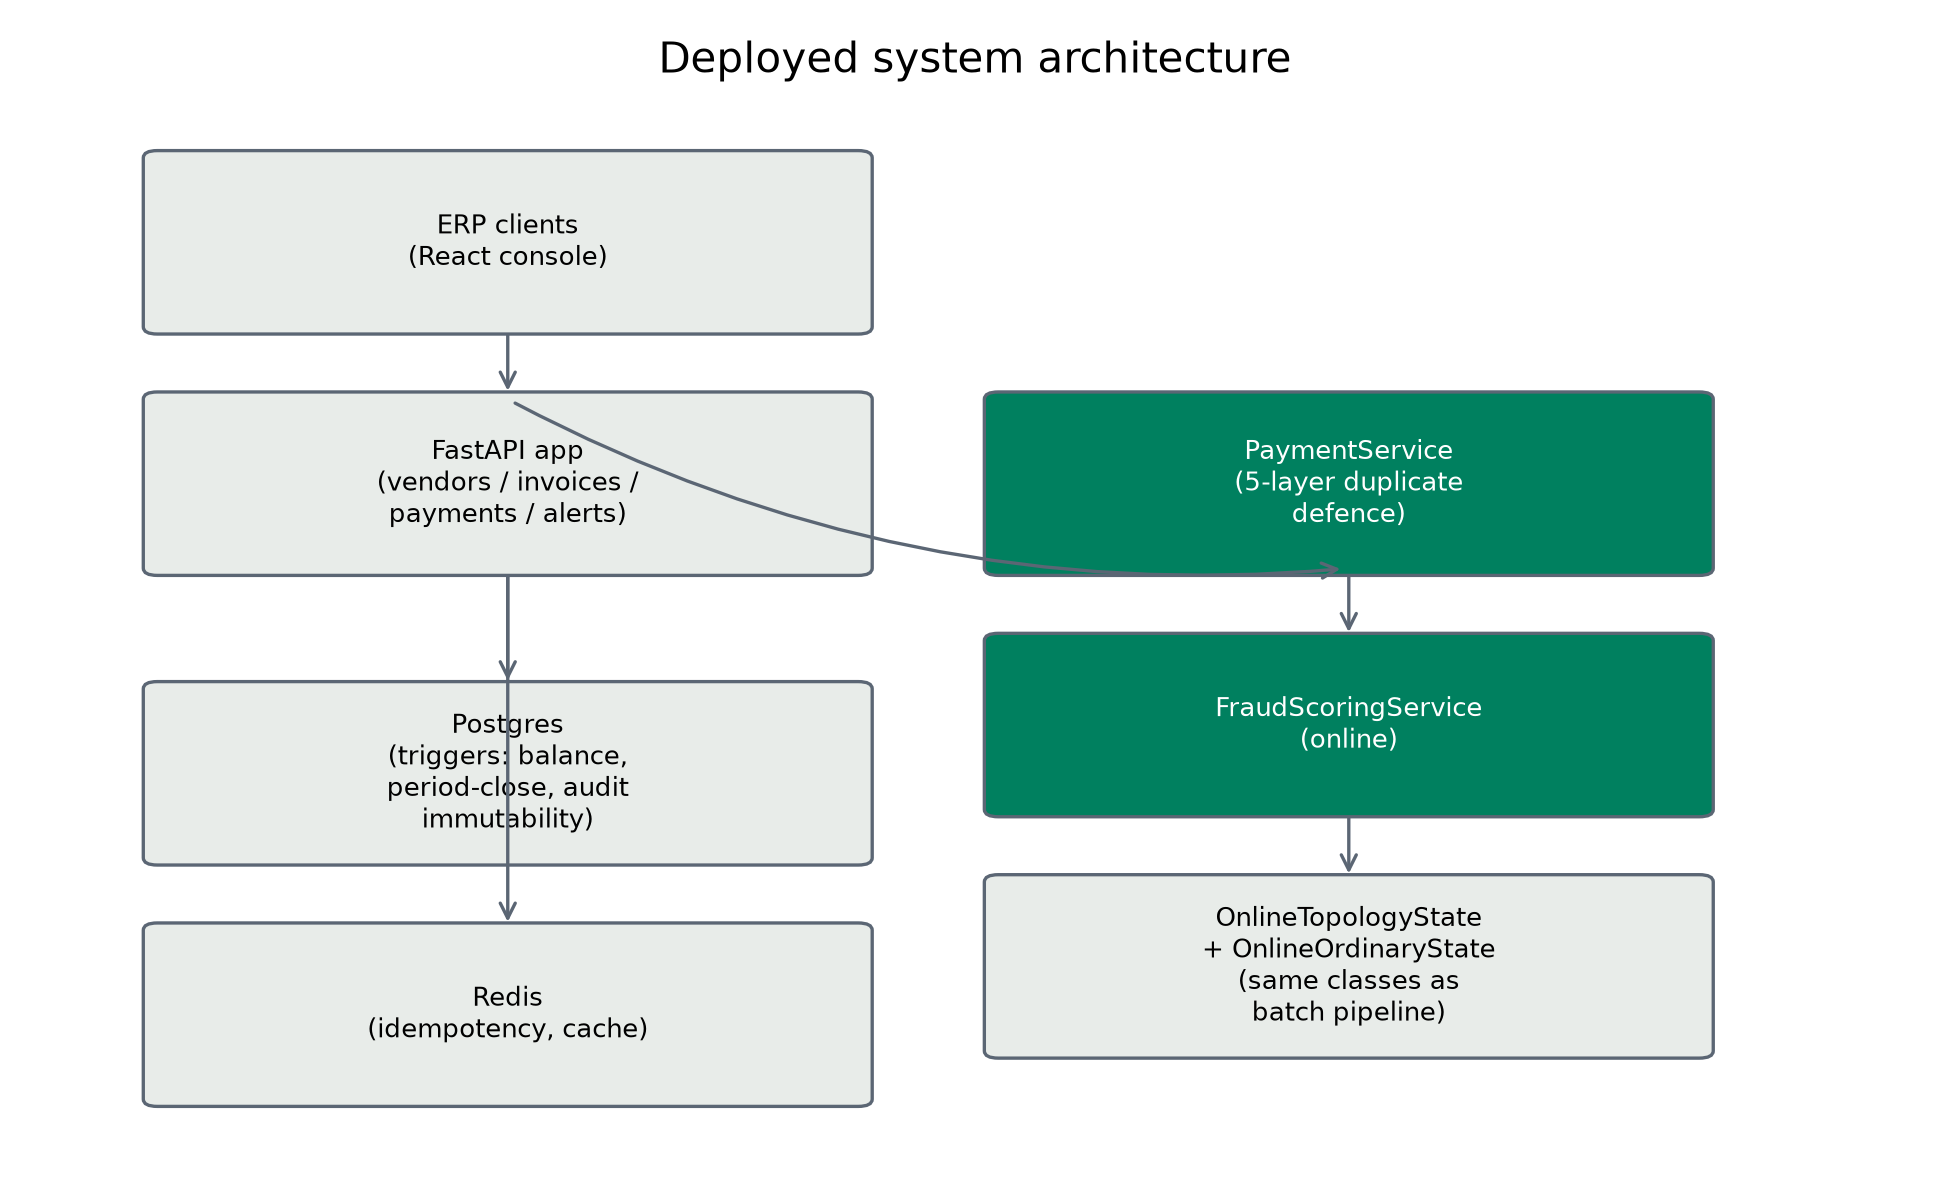
\includegraphics[width=\columnwidth]{figures/system_architecture.png}
  \caption{Deployed system architecture. The online \texttt{FraudScoringService} reuses the research pipeline's \texttt{WindowGraph}/\texttt{LapMemory} classes directly rather than a reimplementation; the offline TGN training path (Section~V) is not part of the serving runtime.}
  \label{fig:architecture}
\end{figure}

Correctness of the reuse, not merely its existence, is what makes the online path trustworthy: \texttt{tests/test\_online\_topology\_parity.py} replays 20{,}000 real transactions through both the batch \texttt{extract\_features} loop and \texttt{OnlineTopologyState.score\_transaction}, asserting every one of the thirteen topology feature columns matches exactly, row for row, with zero mismatches. The read-then-insert ordering inside the online class is copied line-for-line from the batch engine specifically to preserve this guarantee — the online driver differs only in holding one graph and two lap-memory instances alive across calls instead of discarding them after a single DataFrame pass.

\subsection{The Online/Offline Serving Gap}\label{sec:system-serving}

The champion models evaluated earlier in this paper (Section~V) include a Temporal Graph Network (TGN) embedding stage~\cite{rossi2020temporal} feeding an XGBoost head~\cite{chen2016xgboost}. These champions are \emph{not} servable online, and the paper makes no claim that they are. Two independent problems rule it out. First, TGN inference requires a memory tensor built by replaying a transaction sequence through the trained network; nothing in this build persists that tensor, so scoring a single live transaction would require replaying the dataset's entire prior history on every request — the opposite of the online engine's O(1)-per-feature design. Second, and more fundamentally, TGN training on this codebase is not bit-reproducible across machines even with a fixed seed: re-running \texttt{modeling.tgn} on freshly downloaded, same-source data and re-scoring against the committed champion bundle diverges substantially (documented in \texttt{docs/BUILD\_SPEC.md} as a reproduction failure on both banksim and sap\_wurzburg test folds), because small floating-point differences in CPU training compound over epochs through a component that accounts for 17--42\% of the champion's feature importance. A component that will not reproduce its own training run on the same machine is not a component a production system should be handed authority to persist and reload.

The deployed artifact is therefore a deliberately smaller "online" bundle, trained on ordinary and topology features only, with the TGN family dropped entirely rather than approximated. This is verifiable directly in the two bundle manifests: the online bundle's feature count is, dataset by dataset, exactly the ordinary-plus-topology subtotal of the champion's own feature-family breakdown (banksim: $21+13=34$; sap\_wurzburg: $20+13=33$; synth\_erp: $15+13=28$; against champion totals of 99, 98, and 93 respectively, each with 65 TGN dimensions removed) — confirming the online bundle is the champion's own feature set with TGN excised, not an independently retrained approximation. Table~\ref{tab:online-gap} reports what that exclusion costs in test PR-AUC, computed directly from \texttt{paper/data/final\_champions.json} (champion) and \texttt{paper/data/online\_bundles.json} (online).

\begin{table}[t]
  \centering
  \small
  \caption{Test PR-AUC: offline TGN-inclusive champion vs.\ the deployed online (ordinary+topology only) bundle, same dataset instance, 3 seeds each.}
  \label{tab:online-gap}
  \begin{tabular}{lccc}
    \toprule
    Dataset & Champion & Online & Gap \\
    \midrule
    banksim      & $0.93637 \pm 0.00154$ & $0.93114 \pm 0.00045$ & $0.00523$ \\
    sap\_wurzburg & $0.1557 \pm 0.07166$  & $0.10939 \pm 0.01982$ & $0.04631$ \\
    synth\_erp    & $0.77845 \pm 0.00526$ & $0.57018 \pm 0.01744$ & $0.20827$ \\
    \bottomrule
  \end{tabular}
\end{table}

The cost of going online is small on banksim (0.005 PR-AUC) but is not uniformly small: synth\_erp pays roughly 0.21 PR-AUC and sap\_wurzburg roughly 0.05, consistent with a component contributing 17--42\% of feature importance being removed entirely. sap\_wurzburg's champion figure also carries the small-test-fold caveat attached to that dataset elsewhere in this paper — both its ablation split and its champion split contain only 25 fraud cases in the test fold, so both the champion and online numbers for that dataset should be read as high-variance point estimates, not precise costs. IBM AML is deliberately omitted from Table~\ref{tab:online-gap}: the champion figure in \texttt{final\_champions.json} (\texttt{ibm\_aml}, PR-AUC $1.0\pm0.0$, consistent with the baseline-saturation finding reported elsewhere in this paper) is trained on a different underlying data acquisition than \texttt{ibm\_aml\_kaggle} (PR-AUC $0.512\pm0.06743$), the fresh Kaggle re-download the online bundle is actually trained and served on. Reporting a "gap" between two different simulator instances would misstate the cost of removing TGN as the cost of a different dataset entirely, so no such number is reported; \texttt{ibm\_aml\_kaggle}'s figure stands on its own as the deployed bundle's performance on the data it was actually built from.

A second, smaller and more deliberate divergence exists between the two paths' ordinary-feature computation. The batch engine's expanding per-account z-score uses the textbook two-pass variance formula ($\overline{x^2} - \bar{x}^2$), which suffers catastrophic cancellation for accounts whose historical amounts are nearly identical — verified on the full banksim dataset to produce spurious $|z|>1000$ values (observed up to $\sim\!10^8$) on 1{,}238 of 594{,}643 rows (0.21\%), where a numerically stable computation should return a near-zero or undefined value. \texttt{app/services/online\_ordinary.py} computes the same statistic via Welford's algorithm, which does not exhibit this failure mode and instead returns \texttt{NaN}. Rather than reproduce a known instability from the locked research pipeline into new serving code for the sake of train/serve identity, the online path uses the numerically correct formulation and accepts a small, disclosed, and precisely quantified skew on 0.21\% of rows as the honest cost of not shipping a bug on purpose.

\subsection{Financial Integrity as Database-Enforced Invariants}\label{sec:system-integrity}

An audit console is only as trustworthy as the ledger it reads from, and a recurring theme in ERP-integrity failures is that correctness logic lives entirely in application code that a bug, a bypassed service layer, or a future direct-SQL script can silently violate. This system treats three financial invariants as properties the database itself refuses to break, implemented as Postgres triggers (\texttt{alembic/versions/6192dae4f4a4\_gl\_invariants\_triggers.py}) rather than API-layer checks alone:

\begin{itemize}
  \item \textbf{Double-entry balance.} A \texttt{DEFERRABLE INITIALLY DEFERRED} constraint trigger on \texttt{journal\_lines} sums debits and credits per \texttt{journal\_entry\_id} and raises at \texttt{COMMIT}, not after each inserted line — necessary because a multi-line entry inserts its debit and credit rows separately and would fail a per-row check on every legitimate entry.
  \item \textbf{Period close.} An ordinary \texttt{BEFORE INSERT OR UPDATE} trigger on \texttt{journal\_entries} rejects any entry referencing a \texttt{fiscal\_period} whose status is not \texttt{open}. A FastAPI-level check exists purely to return a friendly \texttt{409} before the raw database exception would; the trigger is the actual enforcement.
  \item \textbf{Audit-log immutability.} \texttt{UPDATE} and \texttt{DELETE} on \texttt{audit\_log} are rejected outright by trigger, unconditionally. Only \texttt{INSERT} is a valid operation — the append-only property a SOX-style audit trail requires is a database guarantee here, not an application convention that a careless migration could quietly undermine.
\end{itemize}

Duplicate-payment prevention receives the same defense-in-depth treatment, layered so that no single control is trusted alone (\texttt{app/services/payment\_service.py}). An idempotency-key middleware replays the stored response for a retried request with the same key rather than re-executing it. Independently, \texttt{create\_payment} takes a \texttt{SELECT ... FOR UPDATE} row lock on the target invoice \emph{before} checking for an existing active payment, closing the check-then-act race that two \emph{different} idempotency keys targeting the same invoice would otherwise open — the scenario a retry-only defense cannot cover, since it is two independent actors, not one repeated request. A partial unique index (\texttt{uq\_payments\_invoice\_live}, Module 3) is the database-level backstop if both application layers are ever bypassed. A \texttt{pg\_advisory\_xact\_lock} per vendor serializes an entire payment run, not just one invoice at a time. Finally, \texttt{tools/reconcile\_payments.py} is a periodic sweep that treats any invoice with more than one non-void payment as an incident — the tripwire for "we were wrong somewhere," not a preventive control. Table~\ref{tab:reliability} reports the formalized, automated test of this defense under real concurrency.

\subsection{Measured Performance, Concurrency, and Recovery}\label{sec:system-performance}

Query optimization was driven by captured \texttt{EXPLAIN (ANALYZE, BUFFERS)} plans against a reproducibly bulk-seeded dev database (5{,}000 vendors, 40{,}000 invoices, 23{,}929 payments, 5{,}000 audit alerts; seed 42; \texttt{ANALYZE} re-run after load so planner statistics are current), not guessed indexes. Table~\ref{tab:queries} reports the result honestly, including the one index that did not help: a composite index added to the vendor-scoped invoice listing on the expectation that it would repeat the first query's win did not change the query plan at all, because at this dataset's distribution (roughly 8 invoices per vendor) sorting that few rows is already cheaper than the planner switching indexes. It remains in the schema — cheap to maintain, and the correct choice the moment a single vendor's invoice volume becomes skewed — but is reported as a non-win rather than silently dropped or claimed as a success it was not.

\begin{table}[t]
  \centering
  \scriptsize
  \resizebox{\columnwidth}{!}{%
  \begin{tabular}{lp{4.3cm}p{4.1cm}c}
    \toprule
    Query & Before & After & Speedup \\
    \midrule
    Paid invoices, newest-first (\texttt{status='paid'} \texttt{ORDER BY invoice\_date DESC LIMIT 50}) &
      Bitmap Heap Scan $\to$ top-$N$ heapsort; 875 buffer hits; 6.331~ms &
      Index Scan Backward, no sort; 50 buffer hits; 0.301~ms & $\sim\!21\times$ \\
    \addlinespace
    Alert queue (\texttt{ORDER BY score DESC LIMIT 50}) &
      No index existed; seq-scan-and-sort baseline never captured at scale\textsuperscript{a} &
      Index Scan (DESC); 0.236~ms & --- \\
    \addlinespace
    Vendor-scoped invoices (\texttt{vendor\_id=?} \texttt{ORDER BY id LIMIT 50}) &
      Bitmap Index Scan on \texttt{vendor\_id} + small sort; 0.253~ms &
      \emph{Same plan} -- new composite index not selected; 0.317~ms & none \\
    \bottomrule
  \end{tabular}}
  \caption{Module 7 query optimization, before/after \texttt{EXPLAIN (ANALYZE, BUFFERS)} on a bulk-seeded dev database. Row 3 is reported as a genuine non-win, not silently dropped.}
  \label{tab:queries}
\end{table}
\vspace{-0.6em}
{\scriptsize\textsuperscript{a}The \texttt{audit\_alerts} table was empty during earlier module testing; no pre-index baseline exists at production row counts, so degradation was inferred, not measured.\par}

Redis-backed response caching (route+params+tenant+role key, ETag/304 support, explicit invalidation on write) and all four new indexes ship as ordinary \texttt{CREATE INDEX} migrations rather than \texttt{CONCURRENTLY} builds — an acceptable simplification against an empty or lightly loaded dev-scale table, but a production rollout against a live, concurrently written table should use \texttt{postgresql\_concurrently=True} outside a transaction block to avoid holding write locks for the duration of the index build.

Observability runs as a verified Prometheus/Grafana/Uptime Kuma stack, not a planned one. Prometheus scrapes \texttt{/metrics} every 10~seconds with the \texttt{shadow-ledger-api} target confirmed healthy; a Grafana dashboard ("Shadow Ledger — Overview") is auto-provisioned alongside the datasource and exposes request rate and 5xx rate by route, p95 latency by route, fraud-scoring latency p50/p95/p99, cache hit rate, and duplicate-payment attempts. \texttt{fraud\_scoring\_latency\_seconds\{dataset\}} is the histogram the paper's sub-200~ms p95 latency target is measured against, reflecting the online path's O(1)-per-feature design (Section~\ref{sec:system-serving}): topology lookup, Welford-based ordinary features, one small XGBoost \texttt{DMatrix} predict, and TreeSHAP, with no whole-stream replay on the request path. Uptime Kuma probes \texttt{/health} and \texttt{/ready} every 30~seconds; \texttt{/ready} already returns 503 the instant the database, Redis, or the scoring registry is unavailable, so the monitor's job is only to alert on a non-200, not to implement the health logic itself. Error logging is structured JSON with correlation-id propagation from the access log through every service call (\texttt{app/core/logging.py}), live since the project's first module and the actual mechanism every bug found during query optimization and testing was diagnosed from; a self-hosted GlitchTip instance was scoped but not deployed, since it requires its own Postgres database, Redis, and Celery worker rather than a docker-compose add-on line — \texttt{GLITCHTIP\_DSN} is already read by \texttt{app/core/config.py} as a drop-in point once a target instance exists.

Concurrency, load, and recovery were exercised as k6 scripts and a scripted backup/restore drill, with every figure below taken from an actual run (\texttt{docs/TESTING\_MODULE9.md}), not a projection. The duplicate-payment race (\texttt{tests/load/payment\_race.js}) is the automated form of the defense in Section~\ref{sec:system-integrity}: 30 virtual users fire truly concurrent payment requests at one invoice, each with a distinct idempotency key, so that the only thing standing between them and a double payment is the row lock and unique index, not idempotency replay. The mixed-workload ramp (\texttt{tests/load/mixed\_workload.js}) drives a 70\%~browse / 20\%~invoice-submission / 10\%~alert-queue-read mix from 0 to 500 concurrent users against a single dev-mode \texttt{uvicorn} process with no worker pool and a 40-connection database pool, deliberately reported as a degradation-point measurement rather than a pass/fail gate.

\begin{table}[t]
  \centering
  \scriptsize
  \caption{Module 9 concurrency and recovery drills — measured results.}
  \label{tab:reliability}
  \begin{tabular}{p{0.22\columnwidth}p{0.36\columnwidth}p{0.32\columnwidth}}
    \toprule
    Drill & Configuration & Result \\
    \midrule
    Duplicate-payment race & k6, 30 VUs, 1 invoice, distinct idempotency keys & 1/30 succeeded, 29/29 rejected (\texttt{duplicate\_payment}); DB confirms exactly 1 payment row; successful-request latency avg 267\,ms, p95 807\,ms \\
    \addlinespace
    Mixed workload ramp & k6, 0$\to$50$\to$200$\to$500 VUs, single uvicorn worker, 40-conn.\ DB pool & 39{,}727 requests attempted, 28{,}642 completed; overall p95 8.18\,s; error rate 4.42\% ($<$5\% threshold passed; $p95<1$\,s threshold \textbf{failed}) \\
    \addlinespace
    Backup/restore drill & \texttt{pg\_dump -Fc} $\to$ clean throwaway DB; row-count + payment-total fingerprint compare & Quiescent run: match=true, RTO$=3.07$\,s (dump 0.95\,s/6.99\,MB, restore 2.12\,s); a run taken concurrently with active writes legitimately reports match=false (Postgres MVCC), reproduced again in the most recent committed drill \\
    \bottomrule
  \end{tabular}
\end{table}

The mixed-workload result is reported as found: the system clearly degrades before reaching 500 concurrent users, with I/O timeouts appearing during the highest-VU stage and overall p95 latency an order of magnitude above the 1-second threshold. This is expected of a single dev-mode process and is the useful output of the test — it names horizontal scaling (\texttt{--workers~N}, a larger pool, or multiple instances behind a load balancer) as the concrete next step for a production rollout, rather than asserting a latency number the current deployment configuration cannot support. The backup/restore drill's own history is a second methodology finding worth stating rather than hiding: an initial drill run taken while the mixed-workload test was still writing to the database correctly reported a fingerprint mismatch, not because backup or restore is broken, but because \texttt{pg\_dump} does not block concurrent writers under Postgres MVCC, so a fingerprint query issued moments before the dump can legitimately diverge from what the dump itself captures. The most recently committed drill artifact (\texttt{infra/backups/last\_drill\_report.json}) reproduces exactly this pattern (match=false, RTO 2.85\,s) against live traffic, while the clean, quiescent-database run reported in Table~\ref{tab:reliability} passed. The operational implication is direct: a production backup schedule needs either a quiescent window, a shared \texttt{pg\_export\_snapshot()}, or reliance on the continuous WAL archiving already enabled (\texttt{archive\_mode=on}) for point-in-time recovery — none of which this session exercised end-to-end, and all of which are named as the concrete next drill rather than assumed solved.

Taken together, these results describe a system whose financial-integrity guarantees are enforced below the application layer, whose online scoring path is provably identical in computation to the offline research pipeline it borrows from (short of the TGN component it deliberately excludes), and whose performance and failure characteristics are measured and disclosed rather than asserted — including the two places (the vendor-index non-win, the sub-500-VU degradation point) where the honest answer is a negative result.